\documentclass[aspectratio=169,10pt]{beamer}

%beamer customization
\usetheme{Montpellier}
\useinnertheme{circles}
\useoutertheme{smoothbars}
\usecolortheme{beaver}
\usepackage{bookman}

\setbeamertemplate{caption}[numbered]
\setbeamercovered{transparent} 

\title{L3E}
\subtitle[L3E]{Libre, Linux, \& \LaTeX \space in Education}
\author[l3eteam]{\textbf{P N Bala Subramanian} \\ \textbf{Sreekanth V K} \\ \textbf{Sumesh K S}}
\logo{
\includegraphics[scale=0.05]{imagens/nitc_logo.png}} 
\institute[citra]{Centre for Information Technology Research and Automation\par National Institute of Technology Calicut \\ supported by \\ FOSS United } 


\usepackage[utf8]{inputenc}
\usepackage[english]{babel}
\usepackage[T1]{fontenc}
\usepackage{tikz}
\usetikzlibrary{shapes,backgrounds}
\usetikzlibrary{decorations.text}


\usepackage{amsmath}
\usepackage{amsfonts}
\usepackage{amssymb}
\usepackage{graphicx}



\begin{document}
	\begin{frame}
		\titlepage
	\end{frame}

    \begin{frame}{About FOSS United}
        \section{FOSS United}
        %\frametitle{FOSS United}
            \begin{columns}
                \begin{column}{0.5\textwidth}
                \begin{itemize}
                    \item FOSS United is a non-profit foundation that aims at promoting \& strengthening the Free and Open Source Software (FOSS) ecosystem in India.
                    \item Read more at:   \href{https://fossunited.org/}{https://fossunited.org/}
                \end{itemize}
                        
                        
                \end{column}
                \begin{column}{0.5\textwidth}
                        
\includegraphics{imagens/fossunited.png}
                \end{column}                
            \end{columns}

    \end{frame}
    
	\begin{frame}{Outline}
		\section{Outline}
		% \frametitle{Outline}
		\begin{itemize}
			\item Day I
			\begin{itemize}
				\item Introduction to Libre and Linux
				\item Introduction to Ubuntu Desktop
			\end{itemize}
			\item Day II
				\begin{itemize}
					\item File Management
					\item Regular Expressions
				\end{itemize}		
			\item Day III
				\begin{itemize}
					\item Shell Scripting
					\item Linux in Daily Life
				\end{itemize}
		\end{itemize}
	\end{frame}
	
	\begin{frame}{Introduction to Libre and Linux}
		\section{Introduction to Libre and Linux}
		%\frametitle{Introduction to Libre and Linux}
		\begin{itemize}
			\item A brief history of Unix \& C - Dennis Ritchie \& Ken Thompson
			\item GNU - GNU is Not Unix - Richard Stallman
			\item Linux - Linus Torvalds
            \item Concept of Libre/Free
			\item Why is it important? 
            \item Opportunities and Challenges
		\end{itemize}
		
	\end{frame}

	\begin{frame}{Introduction to (GNU)Linux}
		%\frametitle{Introduction to (GNU)Linux}
        \begin{columns}
            \begin{column}{0.5\textwidth}
                \begin{itemize}
                    \item Multi-User and Multi-Tasking 
                    \item Linux Architecture
                    \begin{itemize}
                        \item Hardware
                        \item Kernel
                        \item Shell
                        \item Utilities / Applications
                    \end{itemize}
                    \item Linux Variants
                    \begin{itemize}
                        \item GNU Variants
                        \item Debian - Ubuntu
                        \item Red Hat
                        \item Suse
                        \item Arch Linux
                        \item Gentoo
                        \item and many more. 
                    \end{itemize}                        
                \end{itemize}
            \end{column}
        \begin{column}{0.5\textwidth}  %%<--- here
            \begin{center}
                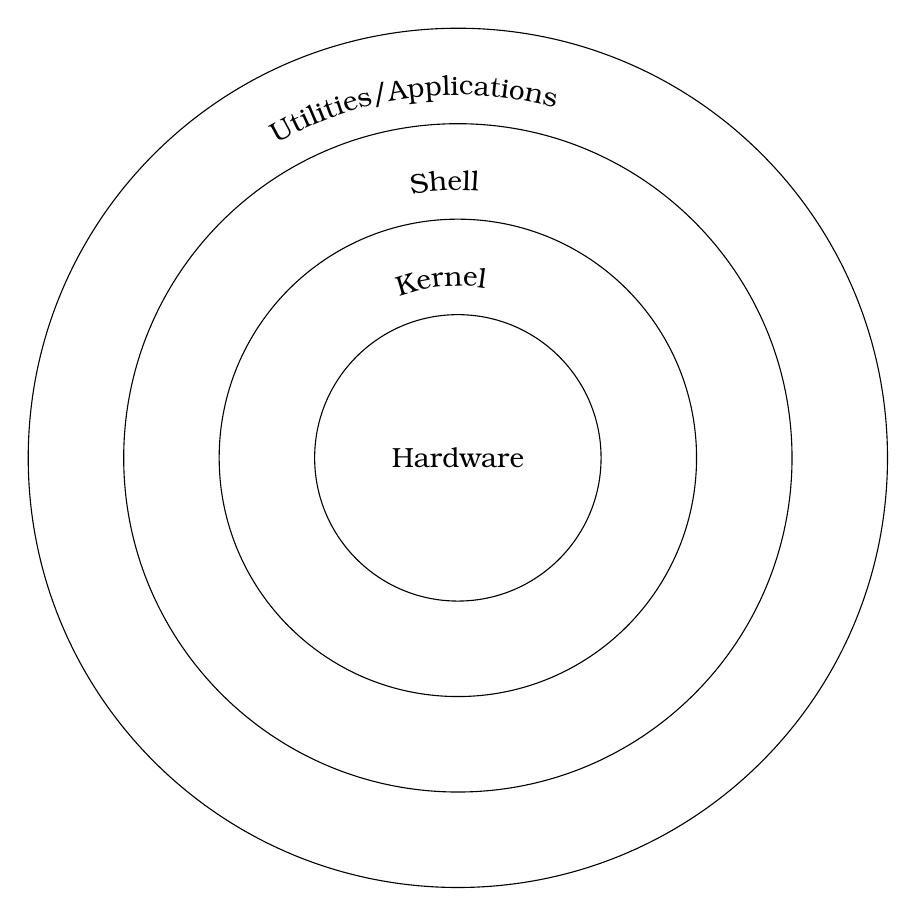
\begin{tikzpicture}
                    \node[circle, minimum size=0.9\textwidth, draw] (a) {};
                    \node[circle, minimum size=0.7\textwidth, draw] (b) {};
                    \node[circle, minimum size=0.5\textwidth, draw] (c) {};
                    \node[circle, minimum size=0.3\textwidth, draw ] (d) {Hardware};

                    \draw [decorate, decoration={text along path, text = Kernel}] (110:0.18\textwidth) arc (110:0:0.18\textwidth);
                    \draw [decorate, decoration={text along path, text = Shell}] (100:0.28\textwidth) arc (100:0:0.28\textwidth);
                    \draw [decorate, decoration={text along path, text = Utilities/Applications}] (120:0.38\textwidth) arc (120:0:0.38\textwidth);                        
                \end{tikzpicture}               
            \end{center}
        \end{column}
        \end{columns}
	\end{frame}
 
    \begin{frame}{Introduction to (GNU)Linux}
        \begin{columns}
            \begin{column}{0.5\textwidth} 
                \begin{itemize}
                    \item Desktop version and Server Version 
                    \item Graphic User Interface and Terminal-based
                    \item Desktop Environments
                    \begin{itemize}
                        \item KDE Plasma, GNOME,  XFCE, MATE, Budgie, LXDE, LXQt, Deepin, and many more
                    \end{itemize}
                    \item Linux window managers
                    \begin{itemize}
                         \item i3, sway, OpenBox, KWin, IceWM, and many more
                    \end{itemize}  

                \end{itemize}
            \end{column}
            \begin{column}{0.5\textwidth} 
                
            \end{column}
        \end{columns}   
    \end{frame}

    \begin{frame}{Introduction to (GNU)Linux}
       \begin{itemize}
            \item Benefits
            \begin{itemize}
                \item Security and Privacy
                \item Control and Freedom
                \item Backup
                \item Choices - based on your hardware as well
                \item Availing community support and contribute to community
            \end{itemize}
            \item Challenges
            \begin{itemize}
                 \item Learning curve
                 \item Taking responsibility
                 \item Effort required for specific customization
            \end{itemize}  
        \end{itemize}
    \end{frame}

    \begin{frame}{Introduction to Ubuntu}
    \section{Introduction to Ubuntu}
       \begin{itemize}
            \item Benefits
            \begin{itemize}
                \item Security
                \item Control and Freedom
                \item Backup
                \item Choices - based on your hardware as well
                \item Availing community support and contribute to community
            \end{itemize}
            \item Challenges
            \begin{itemize}
                 \item Learning curve
                 \item Taking responsibility
                 \item Effort required for specific customization
            \end{itemize}  
        \end{itemize}
    \end{frame}


\end{document}